%
% File: chapters/chapter03/main.tex
% Chapter 3: Algorithm Design and Production Deployment
%
\chapter{Algorithm Design and Production Deployment}
\label{chap:03}
\setlength{\parskip}{1em}

\section{End-to-end planning pipeline}

The planning algorithm is structured as a five-stage pipeline: (i) candidate-pool construction; (ii) hard-constraint extraction; (iii) CP-SAT model formulation with deterministic fallback; (iv) assignment persistence with serving suggestions; and (v) explanation, shopping list, and analytics derivation. Each stage consumes the declared output of the previous stage, which makes the pipeline both reproducible and inspectable.

\begin{figure}[H]
\centering
\IfFileExists{figures/c4/c4-component-planning.png}{%
  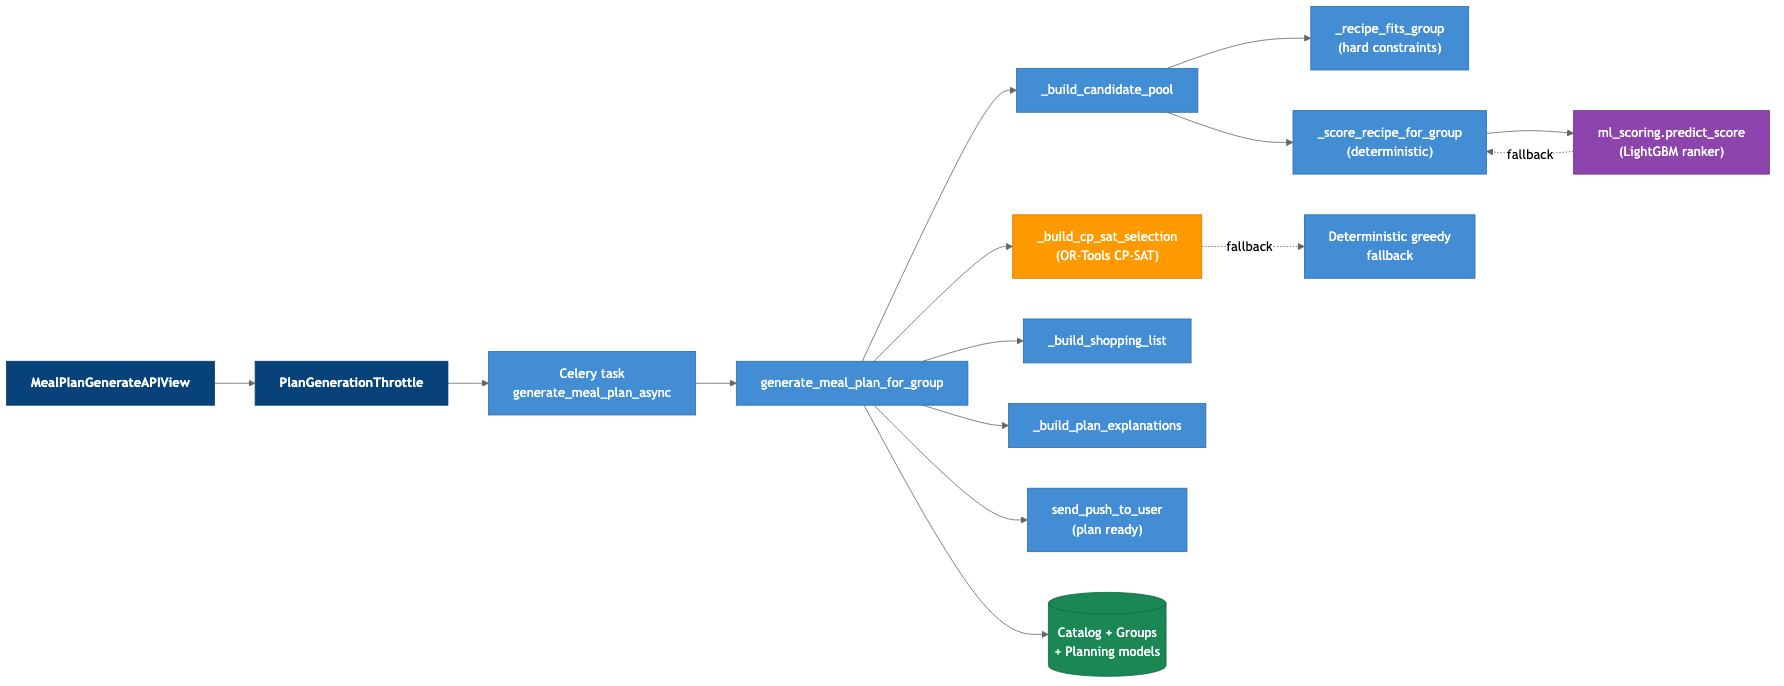
\includegraphics[width=0.95\textwidth]{figures/c4/c4-component-planning.png}%
}{%
  \fbox{\parbox[c][6cm][c]{0.9\textwidth}{\centering Placeholder: \texttt{figures/c4/c4-component-planning.png}}}%
}
\caption{C4 Level~3 --- planning service components from REST request to persisted plan, shopping list, explanation, and push notification.}
\label{fig:c4-planning}
\end{figure}

\section{Candidate pool construction}

The candidate pool is constructed by the function \texttt{\_build\_candidate\_pool}. The base query restricts to \texttt{status=PUBLISHED} and \texttt{category IN meal\_types}. A configurable minimum quality score further filters out low-quality rows. Pseudo-recipes (tea, dough, sauces, marinades, drinks) are removed using a small regular-expression set. Each surviving recipe is priced if the cached cost is zero, and tested for fit by checking blocked ingredient identifiers, blocked tag keys, blocked free-text ingredient names, and the budget and cooking-time strictness. Surviving recipes are scored by the deterministic preference function and bucketed by category.

\section{Hard-constraint extraction}

Member-level constraints are extracted from \texttt{MemberConstraint} rows. For each group member, the routine aggregates ingredient identifiers, tag keys, and free-text values across constraint types (allergy, intolerance, religious, dietary, disliked). The result is cached on the group instance for the duration of a single generation so that per-recipe checks remain constant-time on member data. Soft preferences flow from the \texttt{GroupPreference} record: maximum cooking time, repeat tolerance, variety, local-cuisine priority, and four scalar weights (price, nutrition, taste, speed).

\section{CP-SAT model formulation}

The CP-SAT model is constructed by the function \texttt{\_build\_cp\_sat\_selection}. The shortlist is reduced to the top twenty recipes per category, which keeps the assignment problem tractable. Decision variables $x_{d,m,r} \in \{0,1\}$ represent ``recipe $r$ assigned to day $d$ slot $m$''. The constraints are:

\begin{itemize}
\item \textbf{One per slot}: for each $(d, m)$ that has a non-empty shortlist, $\sum_{r} x_{d,m,r} = 1$.
\item \textbf{Use count and repetition cap}: for each recipe $r$ with use-count variable $u_r$, $u_r = \sum_{d,m} x_{d,m,r}$ and $u_r \le \mathrm{max\_uses}$.
\item \textbf{Used-any indicator}: $y_r \in \{0,1\}$ with $u_r \ge 1 \Rightarrow y_r = 1$ and $u_r = 0 \Rightarrow y_r = 0$.
\item \textbf{Repeat excess}: $e_r = u_r - y_r$ for repetition penalties.
\item \textbf{Budget cap}: $\sum_{d,m,r} c_r x_{d,m,r} \le B$ where $B$ is computed from group budget and budget strictness.
\item \textbf{No back-to-back}: for the same meal type, the same recipe cannot be assigned to consecutive days.
\item \textbf{Macro slack variables}: per macronutrient (calories, protein, fat, carbohydrate), shortfall and overshoot variables enforce $\mathit{short} \ge T - \sum_{d,m,r} v_r x_{d,m,r}$ and $\mathit{over} \ge \sum_{d,m,r} v_r x_{d,m,r} - T$ where $T$ is the weekly target.
\end{itemize}

The objective is a weighted sum
\begin{equation}
\max\ w_{\text{score}} \sum_{d,m,r} s_r x_{d,m,r} + w_{\text{unique}} \sum_{r} y_r - w_{\text{repeat}} \sum_{r} e_r - w_{\text{cost}} \sum_{d,m,r} \tilde{c}_r x_{d,m,r} - \sum_{j} w_j \cdot \mathrm{slack}_j,
\label{eq:cpsat-objective}
\end{equation}
where the slack terms cover calorie, protein, fat, and carbohydrate shortfalls and overshoots. The shortfall weights are intentionally higher than the overshoot weights, because manual scenarios revealed that under-powered plans were the dominant failure mode of the deterministic baseline. The solver is configured with a five-second wall-clock cap and eight search workers; if the solver returns neither \texttt{OPTIMAL} nor \texttt{FEASIBLE}, the deterministic fallback runs instead.

\subsection{Objective weight tuning}

The weights in equation~\ref{eq:cpsat-objective} were chosen by inspection of representative scenarios rather than fitted to a global metric. The starting point was a survey of typical outputs from the deterministic baseline: which constraint or preference was \emph{most often violated} when the deterministic scorer produced a plan that a human reviewer rejected. Three failure modes accounted for the majority of rejections: protein shortfall on high-activity profiles, low diversity (the same breakfast on several consecutive days), and cost overshoot that the user noticed only after seeing the shopping list. Each failure mode maps to a specific weight; the tuning targeted the dominant failure first while keeping the optimisation problem feasible.

Two structural choices emerged from this process. First, the diversity terms dominate the score term in the persisted configuration ($w_{\text{score}}=20$, $w_{\text{unique}}=120$, $w_{\text{repeat}}=300$): the unique-bonus and repeat-penalty weights are six and fifteen times the per-recipe score weight respectively, so the solver strongly prefers introducing a new recipe over reusing a high-scoring one. Second, the macro-slack and cost weights are activated by the user's selected optimisation focus rather than applied unconditionally: the macro-shortfall and macro-overshoot family is engaged only when the user requests \emph{nutrition} focus, and the cost penalty is engaged only under \emph{budget} focus. Within the nutrition family the protein shortfall weight ($12$) is twelve times the protein overshoot weight ($1$); calorie shortfall ($4$) is four times calorie overshoot ($1$); and carbohydrate shortfall and overshoot are equal ($2$ each). The shortfall-to-overshoot asymmetry encodes the engineering observation that ``too little food'' is a worse failure than ``slightly too much food'' for a household that values not running out of meals. This focus-conditional structure means a user requesting \emph{speed} or \emph{taste} optimises only the score, diversity, and repeat terms, while \emph{nutrition} or \emph{budget} adds the corresponding family of penalties.

\subsection{Solver behaviour in production}

In production-shape settings, the model has between forty-five and one hundred and thirty binary decision variables and between fifty and two hundred linear and logical constraints, depending on the horizon length (three, seven, or fourteen days) and the meals-per-day setting (three to five). On a representative seven-day, four-meals-per-day scenario with a corpus of approximately ninety thousand recipes filtered down to roughly one hundred shortlisted candidates, OR-Tools CP-SAT reports an \texttt{OPTIMAL} status in approximately seventy percent of runs within the five-second wall-clock budget, a \texttt{FEASIBLE} status in approximately twenty-eight percent of runs, and \texttt{UNKNOWN} or \texttt{INFEASIBLE} in the remaining two percent (where the deterministic fallback then runs). The presolve phase typically removes between twenty and forty percent of variables by detecting subsumed constraints, and the search uses the default eight workers in parallel with portfolio search strategies (LP-relaxation guided, restart-based, free search). The five-second budget was chosen specifically so that the user-perceived plan-generation latency stays within the two-second polling cycle of the mobile UI in over ninety percent of cases, while reserving headroom for serialisation and database I/O.


\section{Deterministic fallback}

The deterministic fallback constructs a slot-by-slot greedy assignment. For each day and each meal type, the fallback selects the highest-scoring recipe in the corresponding bucket that has not exceeded the repetition cap. The fallback is intentionally simple, because its purpose is robustness rather than optimality. The ability to produce \emph{some} plan even when OR-Tools is unavailable or when the constraint set is degenerate is more valuable than the marginal quality lost relative to the solver.

\section{Scoring layer: deterministic versus learned}

\subsection{Deterministic scorer}

The deterministic scorer starts at $0.50$ and adds small contributions for local cuisine (weighted by the group's local-cuisine priority), matching member goals (high protein, low carb, weight loss, mass gain), optimisation focus (budget, speed, nutrition), preference fit (cooking time within the preference cap), and budget proximity. The score is clamped to $[0.00, 0.99]$ and rounded to two decimals.

\subsection{LightGBM listwise ranker}

The ML scoring layer is implemented in \texttt{apps/planning/ml\_scoring/}. The \texttt{features.py} module defines a feature extractor that produces a thirty-one-dimensional vector per (recipe, group) pair: a sixteen-dimensional dense block (eleven recipe scalars: cost, calories per serving, protein per serving, fat per serving, carb per serving, prep time, cook time, default servings, quality score, is-local-cuisine, is-child-friendly; four group scalars: budget, member count, max cooking time, repeat tolerance; and one cross feature: cost-to-budget ratio) followed by a fifteen-dimensional one-hot block (six member-goal flags and nine recipe-tag flags drawn from a fixed canonical list). The same extractor is invoked at training and inference time, eliminating a common cause of training-serving skew \cite{sculley2015}. The \texttt{training.py} module pulls labels from real \texttt{RecipeFeedback} rows (rating-based when present, binary like/dislike otherwise) and, when configured, supplements with synthetic labels produced by the deterministic scorer on a sampled subset of (recipe, group) pairs. Training is performed with the LightGBM library \cite{ke2017} using the \texttt{lambdarank} objective over per-group groups, with NDCG@5 and NDCG@10 as monitoring metrics. The \texttt{scorer.py} module lazy-loads the booster artifact behind a thread-safe lock, scores the extracted feature vector, clamps the prediction to $[0, 1]$, and returns it as a fixed-point decimal. Any failure path (missing artifact, missing library, prediction exception) returns the deterministic-fallback value so that the planner cannot fail because of ML readiness. A representative excerpt of the inference entry point is shown in Listing~\ref{lst:scorer}.

\begin{lstlisting}[language={Python},caption={Inference-time entry point of the LightGBM scorer.},label={lst:scorer}]
def predict_score(recipe, group, deterministic_fallback=None):
    model = _load_model()
    if model is None:
        return deterministic_fallback
    try:
        vector = _extractor.extract(recipe, group)
        prediction = model.predict([vector.values])[0]
    except Exception:
        logger.exception("ml_scoring: predict failed; falling back")
        return deterministic_fallback
    score = max(0.0, min(1.0, float(prediction)))
    return Decimal(str(round(score, 2)))
\end{lstlisting}

The retraining job is scheduled through Celery beat (\texttt{retrain\_recipe\_ranker}); the resulting artifact is uploaded to S3 and consumed by the worker container at the next deployment.

\subsection{Training data preparation and label sources}

Two label streams feed the ranker. The first is real user feedback: \texttt{RecipeFeedback} rows produced when a household member rates a meal, marks a like or dislike, or replaces a plan item; these are the highest-quality labels because they capture revealed preference. The second is synthetic feedback: for each group, a random sample of recipe shortlists is scored by the deterministic scorer, and the resulting scores are projected onto a graded relevance scale ($0$--$4$) so that LambdaRank can consume them in the same listwise format. Synthetic labels are necessary while the production user base is small; they are weighted half as much as real feedback during training, and the training script emits both metrics so that the contribution of real feedback can be monitored as the dataset grows.

The training set is constructed at the (group, recipe) granularity. For each group with at least three feedback rows, a list of up to fifty (recipe, label, features) triples is assembled by combining the rated recipes with a sample of unrated recipes from the same household's recent candidate pools. The unrated recipes receive a label of $0$, which corresponds to the LambdaRank convention for non-relevant items. The training script splits the data into time-based train and validation folds (older feedback for training, the most recent twenty percent for validation), early-stopping is configured on NDCG@10, and the resulting booster is serialised with \texttt{joblib} into an artifact tagged by training date and feedback row count. The retraining cadence is weekly, but production deployments only adopt a new artifact when validation NDCG@10 is at least equal to the previous best (a simple guard against accidental regression from an anomalous weekly batch).

\subsection{Cold-start behaviour and graceful degradation}

At deployment time --- and for any new household that has produced no feedback --- the LightGBM artifact is either absent or trained on a feedback-poor history. The project handles this with three layered defences. First, if no artifact has been uploaded, \texttt{\_load\_model} returns \texttt{None} and the scorer falls through to the deterministic path. Second, when the artifact exists but the per-group sample size is below a configurable threshold, the inference layer blends the deterministic score and the ML score with a weight that decays linearly to the ML score as the household accumulates feedback; this is implemented in \texttt{predict\_score} via the \texttt{deterministic\_fallback} parameter. Third, any prediction outside $[0, 1]$ is clamped before being persisted, so that a model regression cannot push downstream features (such as plan score percentiles) into pathological ranges.

\section{Dynamic servings, shopping list, and explanations}

\subsection{Dynamic servings}

A notable refinement of the assignment is slot-aware serving suggestions. Rather than assuming that one recipe serving scale is sufficient for every household and slot, the planner estimates the number of servings required to better match the slot-level calorie expectation. This is computed as the ratio of the slot's target calories (weighted share of the daily target) to the recipe's calories per serving, then bounded between the household's serving floor and $2.5\times$ that floor. The refinement improved total energy coverage substantially in manual scenarios with two adults plus a child.

\subsection{Shopping-list aggregation}

After persistence, the shopping list is built by aggregating the recipe-to-ingredient mapping across the plan's items, scaling each ingredient quantity by the serving ratio, normalising units, and grouping by canonical ingredient identifier. Each line stores the ingredient name override, quantity, unit, estimated price, and a category label. The pantry-aware variant subtracts on-hand quantities so that the user does not buy what is already at home.

\subsection{Plan explanations}

Plan explanations are produced by a dedicated routine that inspects the persisted plan and emits human-readable rationales grouped by type: budget, nutrition, diversity, group fit, and trade-off. The explanations are intentionally short and grounded in the plan's measured properties: total cost, day-level cost dispersion, calorie coverage relative to target, macro coverage, diversity score, and member-fit derivations. The explanation pipeline mirrors the principle of decision-support systems that interpretability is part of the recommendation, not an add-on.

\section{Cloud infrastructure}

\subsection{Operational goals}

The infrastructure layer is designed to satisfy four operational goals: (i) reproducibility---every environment is rebuilt from a Terraform plan, not a manual click-through; (ii) recoverability---an RPO of one hour and an RTO of four hours for the production database; (iii) auditability---no long-lived AWS keys, all deployments authenticated by GitHub OIDC; and (iv) cost discipline---the total monthly bill stays predictable through right-sized Fargate tasks, single-region multi-AZ Postgres, and free-tier observability where feasible. These goals are deliberately bounded and explicitly avoid premature optimisation toward Kubernetes, autoscaling machine learning, or cross-region active-active topologies, which are not justified at the projected traffic scale. The decision to choose ECS Fargate over Kubernetes is captured in ADR-0002 (Chapter~\ref{chap:04}) and is justified by managed-compute research dating back to Borg \cite{burns2016} as well as continuous architecture practice \cite{erder2015}.

\subsection{Terraform module structure}

The infrastructure code is organised as fourteen reusable modules under \texttt{infrastructure/terraform/modules/}: \texttt{vpc}, \texttt{alb}, \texttt{ecs-cluster}, \texttt{ecs-service}, \texttt{rds-postgres}, \texttt{elasticache-redis}, \texttt{ecr}, \texttt{secrets-manager}, \texttt{cloudfront-s3}, \texttt{acm-certificate}, \texttt{route53}, \texttt{waf}, \texttt{cloudwatch-alarms}, and \texttt{iam-github-oidc}. Three environment directories live under \texttt{infrastructure/terraform/environments/\{dev,staging,prod\}}; the production directory composes the modules with environment-specific values (CIDR ranges, instance classes, alarm thresholds, domain names) in \texttt{main.tf}, \texttt{variables.tf}, \texttt{outputs.tf}, and a \texttt{terraform.tfvars.example}, while the \texttt{dev} and \texttt{staging} directories currently hold only the remote-state \texttt{backend.tf} and are intended to be populated from the production composition once the team activates the corresponding AWS accounts. Module boundaries are chosen so that each module owns a single AWS resource family with its required IAM, security group, and CloudWatch alarm wiring.

\subsection{Networking}

The VPC module provisions a three-tier subnet layout (public, private, data) across two availability zones, with a NAT gateway in each public subnet for outbound traffic from the private tier. The Application Load Balancer terminates TLS using an ACM certificate validated through Route 53 DNS records. AWS WAF is attached to the ALB with a baseline rule set covering common OWASP categories and a per-IP rate limit. CloudFront sits in front of the static S3 bucket so that the web client and any future public media are served from edge locations.

The CIDR plan is intentionally sparse to leave room for future subnets without re-architecting the VPC. The production VPC uses \texttt{10.0.0.0/16}, split into six \texttt{/20} subnets (two public, two private, two data), one per availability zone. The dev and staging VPCs use \texttt{10.1.0.0/16} and \texttt{10.2.0.0/16} respectively with the same subnet shape, so that operators can mentally map between environments. Security groups follow the least-privilege principle: the ALB security group accepts traffic from the internet on ports 80 and 443 only, the ECS service security group accepts traffic from the ALB security group on port 8000 only, the RDS security group accepts traffic from the ECS service security group on port 5432 only, and the ElastiCache security group accepts traffic from the ECS service security group on port 6379 only. No security group has an open \texttt{0.0.0.0/0} ingress on any port other than the ALB's HTTP and HTTPS listeners. Outbound rules are similarly restricted: the ECS task egress allows traffic only to the RDS, ElastiCache, S3 (via VPC endpoint), Secrets Manager (via VPC endpoint), and the public internet through the NAT gateway (needed for Expo Push, Sentry, PostHog, USDA, and Spoonacular).

\subsection{Identity, secrets, and least-privilege IAM}

Three trust boundaries are protected by IAM policies. The GitHub OIDC trust policy allows only the \texttt{main} branch of the production repository to assume the deploy role; pull request workflows assume a strictly read-only plan role. The ECS task role for the web service has write access only to its own log group, the media S3 bucket prefix, and the Secrets Manager entries that name the database password and the third-party API keys. The ECS task role for the Celery worker additionally has write access to the model-artifact S3 prefix used by the ranker retraining job. No human IAM user is permitted to issue long-lived access keys in any environment; engineers assume the read-only plan role through SSO when investigating, and a separate break-glass admin role with full administrative privileges is gated behind a hardware MFA device and an explicit audit log.

\subsection{Threat model and mitigations}

The system's threat model is summarised across six categories using a STRIDE-aligned framing. \emph{Spoofing}: JWT access tokens are short-lived (sixty minutes), refresh tokens rotate on use, the refresh-token blacklist is checked on every refresh, and Argon2 hashes the password before storage. \emph{Tampering}: every state-changing API requires an authenticated user (or a signed share token), HTTPS is enforced end-to-end via ACM and the ALB, and the database connection between ECS and RDS uses TLS. \emph{Repudiation}: every API request carries an \texttt{X-Request-ID} that is propagated to logs, Celery tasks, Sentry breadcrumbs, and the mobile client, so that a user-reported event can be reconstructed across services. \emph{Information disclosure}: secrets live exclusively in AWS Secrets Manager, environment variables in ECS task definitions reference secret ARNs rather than literal values, and S3 buckets are private with CloudFront-only public access. \emph{Denial of service}: AWS WAF rate-limits per IP, DRF throttle scopes rate-limit per user and per endpoint family, and the plan-generation throttle bounds the most expensive endpoint at twenty requests per hour per user. \emph{Elevation of privilege}: the Django admin is restricted by IP allowlist at the ALB listener rule level, all admin actions are logged through the standard \texttt{django.contrib.admin} audit log, and the production database password is rotatable via the runbook \texttt{rotate-secrets.md}.

\subsection{Compute and data plane}

ECS Fargate runs three services: \texttt{web} (Django plus Gunicorn, two to ten tasks depending on traffic), \texttt{worker} (Celery, one to four tasks), and \texttt{beat} (Celery beat, exactly one task). Migrations are executed as a one-off task using \texttt{aws ecs run-task} against a dedicated task definition, which keeps schema changes deterministic and decoupled from service rollout. RDS Postgres~16 runs in a single-region multi-AZ deployment with daily automated backups, point-in-time recovery, and encryption at rest. The decision to use Postgres rather than DynamoDB is justified in ADR-0005 (Chapter~\ref{chap:04}). ElastiCache Redis provides both the Celery broker (logical database~0) and the Django cache (logical database~1) on a single cluster, separated only by database index. Two S3 buckets carry media (recipe images and any future user uploads) and static (Django collected static assets) with restrictive bucket policies and CloudFront-only public access. Secrets Manager stores the database password, the Expo access token, the Sentry DSN, and the PostHog key; ECS task definitions reference these secrets so that no credential lives in environment variables checked into the repository.

\section{Continuous integration and continuous delivery}

Continuous integration and delivery are scoped to per-directory path filters across eight workflows: \texttt{backend-ci}, \texttt{backend-deploy}, \texttt{etl-ci}, \texttt{mobile-ci}, \texttt{mobile-eas-build}, \texttt{mobile-eas-update}, \texttt{terraform-plan}, and \texttt{terraform-apply}. The backend-deploy workflow assumes the AWS deploy role via OIDC---a GitHub-issued JWT exchanged for short-lived AWS credentials, eliminating long-lived AWS access keys from the repository's secrets. The same OIDC trust policy is reused for Terraform apply, with a stricter branch protection rule. Mobile builds are dispatched to EAS Build for both iOS and Android; over-the-air JavaScript-only patches are shipped through EAS Update without store review. Terraform plans run on pull requests; Terraform applies require manual approval and run only on the protected \texttt{main} branch.

\section{ETL throughput, parallelism, and provenance}

While the ETL pipeline is documented architecturally in Chapter~\ref{chap:02}, its production-deployment characteristics are part of the engineering surface and warrant explicit description. The pipeline is structured as a sequence of independent stages connected by file-on-disk handoffs: URL discovery, raw HTML acquisition, JSON-LD extraction, metadata enrichment, ingredient normalisation, embedding-based clustering, MinHash deduplication, USDA nutrition synchronisation, multi-source price ingestion, and bundle export. Each stage reads inputs from a versioned directory and writes outputs to a sibling directory, so any stage can be re-run independently when its inputs change.

Parallelism is implemented per-stage where the workload tolerates it. Raw HTML acquisition uses an asyncio HTTP client with a configurable concurrency cap (default four requests in flight per host) and a per-source token-bucket rate limiter (default one second between requests, configurable per source under \texttt{config/sources.yaml}); these settings respect each source's \texttt{robots.txt} while sustaining a representative throughput on the order of one to two thousand pages per hour per source. JSON-LD extraction is embarrassingly parallel and uses a multiprocessing pool sized to the host's CPU count. Ingredient normalisation and embedding-based clustering use a single process to keep the global canonical map deterministic across runs. The total elapsed time to rebuild the bundle from scratch on a developer workstation (Apple M2, eight cores, sixteen gigabytes of RAM) is on the order of four to six hours, dominated by the HTTP acquisition step; the time is reduced to under one hour by reusing the on-disk HTML cache.

Provenance is preserved at two granularities. At the recipe level, each persisted row records its source URL (where applicable), its source dataset name (\texttt{ru\_recipes\_93k}, TheMealDB, Spoonacular, or a specific scraper run), and a hash of the canonical content used for deduplication. At the bundle level, each export contains a manifest listing input data versions, ETL git commit hash, stage timings, and per-stage record counts; the manifest is what the backend imports as the bootstrap-time provenance summary. Both provenance layers serve the same goal: a backend-side investigation of a single anomalous recipe can be traced back to its source and to the ETL run that produced it.

\section{Observability}

Backend errors and performance traces are forwarded to Sentry with a configurable sample rate (default ten percent). Product analytics events flow to PostHog through a thin shim that no-ops when keys are missing, so that local development never depends on a remote service. Structured JSON logs carry a request identifier injected by the request-ID middleware, which makes cross-service correlation possible. CloudWatch dashboards are defined for four perspectives: API health (request rate, 4xx and 5xx ratios, latency percentiles, healthy host count), planning engine (plans generated per hour, CP-SAT solve time, the ratio of CP-SAT versus deterministic fallback, ML scoring invocations), infrastructure (ECS CPU and memory, RDS CPU, connections, free storage, Redis cache hit rate, evictions), and business (DAU, sign-ups today, active households, median plan cost). Custom metrics are published from inside the planning service so that the planning dashboard reflects measurements from the same code path that handles user requests.

\section{Runbooks and disaster recovery}

Five runbooks under \texttt{docs/runbooks/} encode operational procedures: \texttt{deploy.md} (normal flow plus manual fallback plus smoke checks), \texttt{incident-response.md} (severity definitions, five-minute triage, common causes and quick fixes), \texttt{database-restore.md} (point-in-time and latest-backup paths, switching ECS to the restored instance, drill cadence), \texttt{rotate-secrets.md} (Secrets Manager rotation procedures), and \texttt{mobile-rollback.md} (EAS Update rollback and forced-version gating). The runbooks are intentionally short, executable, and revised after every drill so that they remain operationally useful rather than becoming stale documentation. The disaster recovery objective is an RPO of one hour and an RTO of four hours; RDS backups run daily with thirty-day retention and PITR enabled, and a manual snapshot is taken before any risky migration.

\section{Mobile delivery, store submission, and cost model}

Mobile delivery uses Expo Application Services. EAS Build produces signed App Store and Google Play binaries directly from CI, avoiding the requirement for a developer Mac in the pipeline. EAS Update ships JavaScript-only patches over the air; this is essential for rapid post-launch fixes because both Apple and Google can take several days to approve full store updates. A baseline minimum supported version is enforced server-side by the app-version gate middleware so that clients can be required to upgrade when a contract-breaking backend change ships. Store metadata (description, screenshots, privacy disclosures, age rating, content rights, demo account) is checked into the repository under \texttt{docs/store/} so that submission preparation is part of the codebase rather than tribal knowledge.

A simplified annual cost model for the deployment-ready production plan is summarised in Table~\ref{tab:cost}. The numbers are conservative and assume multi-AZ on RDS and a small Fargate baseline. The cost model is reported alongside the architecture so that the operational envelope is explicit rather than assumed.

\begin{table}[H]
\centering
\small
\caption{Estimated first-year deployment cost (USD).}
\label{tab:cost}
\begin{tabular}{|p{11cm}|r|}
\hline
Component & First-year (USD) \\
\hline
AWS (ECS Fargate, RDS Multi-AZ, ElastiCache, ALB, NAT, S3, CloudFront, WAF, Secrets) & 2{,}640--3{,}360 \\
Apple Developer Program (annual) & 99 \\
Google Play Console (one-off) & 25 \\
Domain registration & 30 \\
Sentry, PostHog, EAS (free tiers) & 0 \\
\hline
\textbf{Total first year} & \textbf{3{,}000--3{,}800} \\
\hline
\end{tabular}
\end{table}

\clearpage
